\documentclass[a4paper,10pt]{article}

\usepackage[utf8]{inputenc}
\usepackage[czech]{babel}
\usepackage[left=2cm,top=3cm,text={17cm,24cm}]{geometry}
\usepackage{graphicx}
\usepackage{listings}
\usepackage{multirow}
\usepackage{array}
\usepackage{url}
\renewcommand{\arraystretch}{2.1}

\title{Systém DNS\\
{\bf\large ISA - Laboratorní cvičení č.3}\\
{\bf\large Prokotol ke cvičení}}

\author{Vysoké učení technické v~Brně}

\date{\url{https://github.com/nesfit/ISA/tree/master/lab3-dns}}

\setlength\parindent{0pt}

\begin{document}

{\let\newpage\relax\maketitle}

Jméno a~příjmení:\\
Login:\\
Skupina (číslo nebo čas):\\
Datum:

\section{Služba DNS}
\textbf{1.2} IPv4 adresa serveru {\tt www.vutbr.cz}: \underline{\hspace{5cm}}\\


\textbf{1.3} Adresa lokálního serveru DNS: \underline{\hspace{55mm}}\\
\vskip 0.1em
\hspace*{0.55cm} V~jaké části dotazu DNS je zapsána hledaná doména? \underline{\hspace{35mm}}\\


\textbf{1.4} Je dotazovaný server DNS autoritativní pro danou doménu? \textbf{ANO / NE}\\
\vskip 0.1em
\hspace*{0.55cm} Je typ odeslaného dotazu DNS rekurzivní? \textbf{ANO / NE}\\

\textbf{1.5} Zjištěné informace z~DNS o~doméně \texttt{fit.vutbr.cz}:
\begin{table}[h]
\begin{tabular}{l|c|c|}
\hline
\multicolumn{1}{|l|}{}                                              & Typ záznamu & ~~~~~~~~~~~~~~~~~~~~~ Hodnota ~~~~~~~~~~~~~~~~~~~~~  \\ \hline
\multicolumn{1}{|l|}{E-mail správce DNS zóny fit.vutbr.cz}       &  & \\ \hline
\multicolumn{1}{|l|}{Primární server DNS domény fit.vutbr.cz}    &  & \\ \hline
\multicolumn{1}{|l|}{Sekundární servery DNS domény fit.vutbr.cz} &  & \\
\multicolumn{1}{|l|}{}                                           &  & \\
\multicolumn{1}{|l|}{}                                           &  & \\ \hline
\multicolumn{1}{|l|}{Primární poštovní server domény fit.vutbr.cz} & & \\ \hline
\multicolumn{1}{|l|}{IPv4 adresa serveru www.fit.vutbr.cz}       &  & \\ \hline
\multicolumn{1}{|l|}{IPv6 adresa serveru www.fit.vutbr.cz}       &  & \\ \hline
\end{tabular}
\end{table}

\vspace{-6mm}

% \section{Služba Whois}
% \textbf{2.1} Ve kterém roce byla zaregistrována doména {\tt vutbr.cz}? \underline{\hspace{3cm}}\\

% \textbf{2.2} IP adresa vašeho počítače (rozhraní \texttt{enp2s0}): \underline{\hspace{3.8cm}}\\

% \hspace*{0.55cm} Zjištěná veřejná IP adresa: \underline{\hspace{3.8cm}}\\

% \hspace*{0.55cm} Proč se veřejná adresa neshoduje s nakonfigurovanou adresou?\underline{\hspace{65mm}}\\

% \vskip 2em

% \textbf{2.3} Regionální registrátor (RIR) zodpovědný za daný adresní rozsah: \underline{\hspace{6.2cm}}\\

% \hspace*{0.55cm} Koncový uživatel daného adresního rozsahu: \hspace*{0.2cm}\underline{\hspace{9.2cm}}\\

% \hspace{0.55cm} Rozsah IP adres přidělený koncovému uživateli: \underline{\hspace{4.2cm}} -- \underline{\hspace{4.2cm}}


\section{Konfigurace vlastního serveru DNS}
{\bf 2.9} Výstup příkazu \texttt{dig <vaše doména> soa}:
%\hspace*{0.7cm} Výstup příkazu \texttt{dig <vase domena> soa}:
{
\footnotesize\\

\hspace*{0.8cm}ANSWER SECTION:\\
\vskip 1em

\hspace*{0.8cm}AUTHORITY SECTION:\\
\vskip 1em

\hspace*{0.8cm}ADDITIONAL SECTION:\\
\vskip 1em

}
\hspace*{0.8cm}Výstup příkazu \texttt{dig pcuc.<vaše doména>.cz}:
{
\footnotesize\\

\hspace*{0.8cm}ANSWER SECTION:\\
\vskip 1em

%\hspace*{0.8cm}AUTHORITY SECTION:\\
%
%\hspace*{0.8cm}ADDITIONAL SECTION:\\
%
}
{\bf 2.15} Výstup příkazu \texttt{dig -x 10.10.10.1xx}, kde {\tt xx} je číslo vašeho počítače:
{
\footnotesize\\

\hspace*{0.8cm}ANSWER SECTION:\\
\vskip 1em

\hspace*{0.8cm}AUTHORITY SECTION:\\
\vskip 1em

%\hspace*{0.8cm}ADDITIONAL SECTION:\\
%
}

\textbf{2.21} Doplňte sekvenční diagram popisující posloupnost dotazů při rezoluci DNS. Do diagramu napište jména a~IP adresy serverů DNS, na které dotaz směroval. Využijte výstup z~programu {\tt dig} a~zachycené komunikace v~programu Wireshark.
\\
\\
%\hspace*{0.8cm}Typ rezoluce: % \textbf{ITERATIVNÍ / REKURZIVNÍ}
\begin{figure}[h]
	\centering
	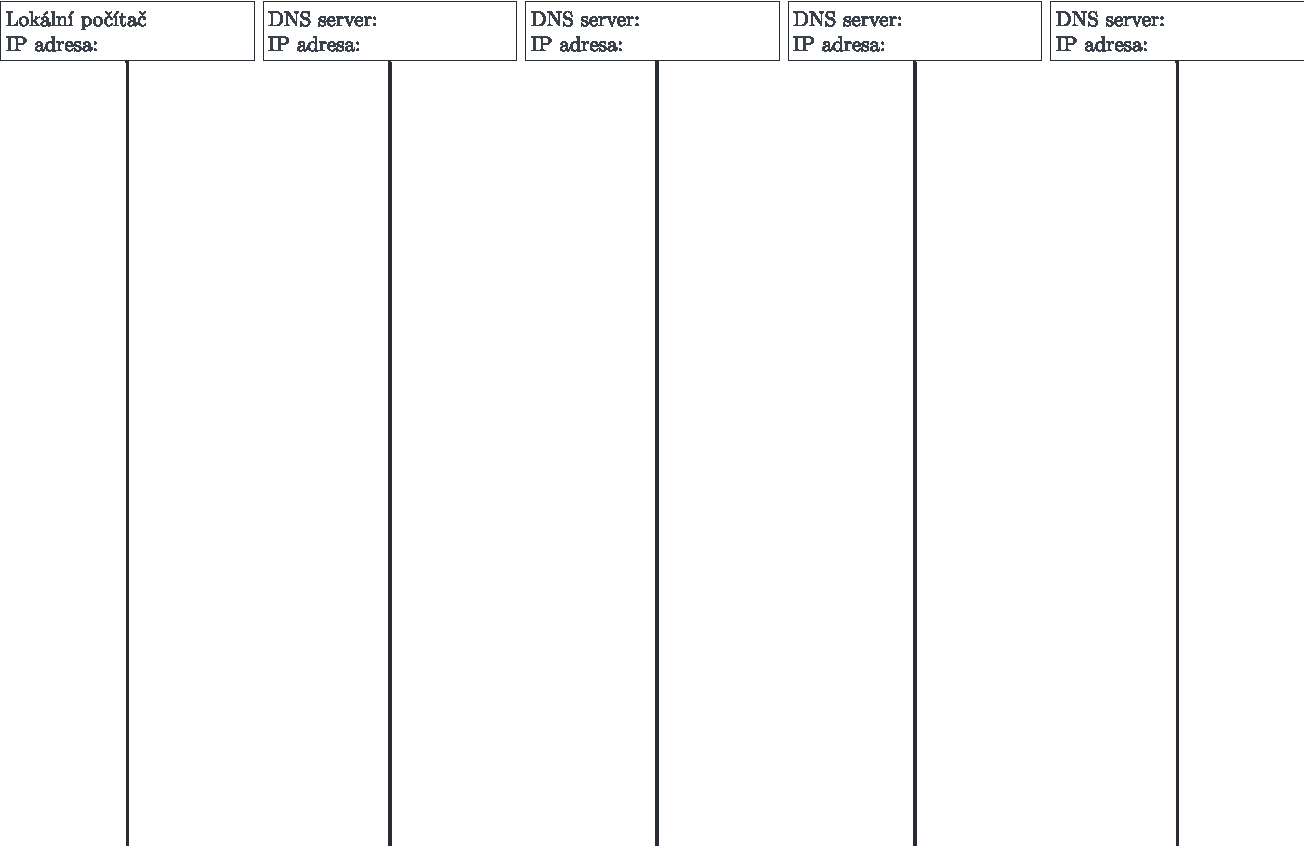
\includegraphics[scale=0.8]{dns-rezoluce.pdf}
%	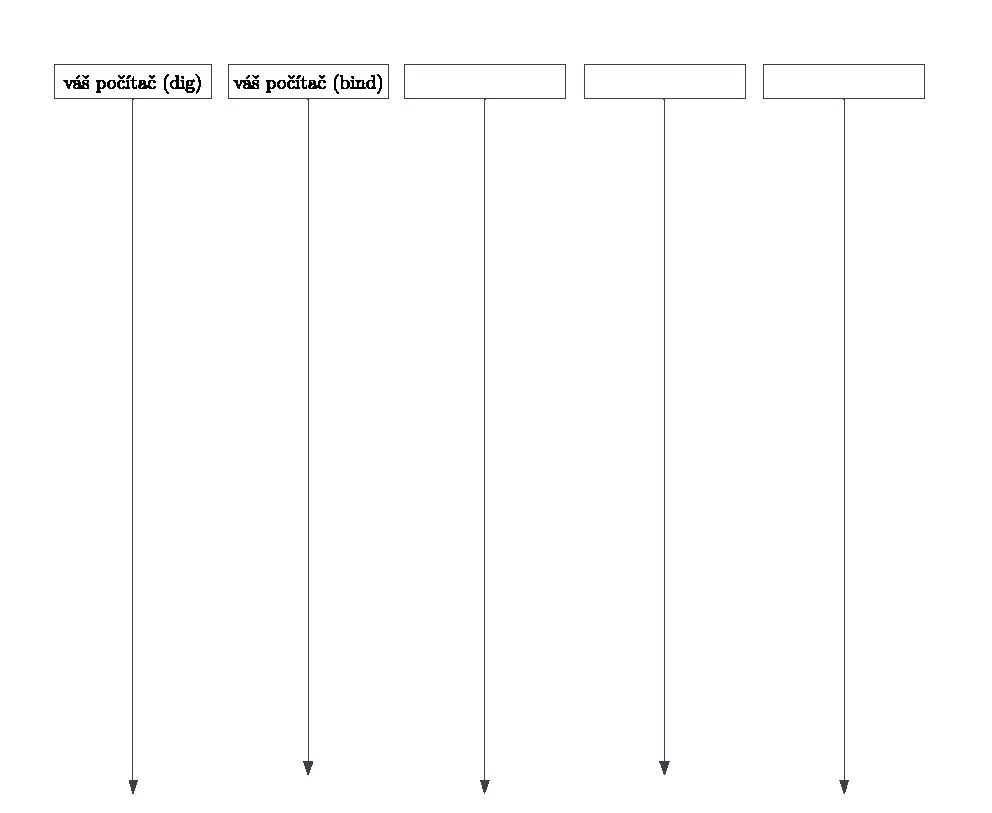
\includegraphics[scale=0.6]{dia.eps}
\end{figure}
%\vskip 0.15em
%\textbf{3.19} Typ rezoluce: \textbf{ITERATIVNÍ / REKURZIVNÍ}\\
%\vskip 0.15em
%\hspace*{0.8cm} Počet vyměněných datagramů na localhost: \underline{\hspace{20mm}}\\
\end{document}
